\chapter{Differentiating between BPMN, CMMN and DMN}
\label{chapter:indicators}

Starting with process management for some companies means to start from the very bottom. They build up their infrastructure, workflows and eventually models on a greenfield. The following sections provide a brief overview of process discovery techniques (manually as well as automated) and serves as an introduction for further reading. It starts with data sources and ends with process maps. Building on process maps and the associated documentation, indicators for the differentiation between BPMN, CMMN and DMN are introduced. Terms and categories will be explained as well as the derivation of each set of indicators along with an explanation of the associated standard. 

\todo{Diagramme mit Legende versehen} 
\todo{Einleitung ins Kapitel erscheint mir noch etwas holprig} 

\section{Discovering the processes}
\label{section:process_discovery}
% Diesen satz kann man gerne woanders wiederverwenden ---- Some researches like Van der Aalst et al. \cite{Aalst2011} put process mining and process discovery on the same semantical level, wherefore different researchers like Laury Verner \cite{Verner2004} don't. 
Processes are resources. Similar to iron or copper, processes lie deep in the bedrock of a company and need to be discovered. This metaphor is not even far-fetched, since the correct terms for gathering information is \textit{process mining} or \textit{process discovery}.
In this chapter, the aggregation of information before the actual process modeling will be discussed, specifically two approaches: A manual one (often referred to as process discovery) and an automated one (often referred to as process mining). Both techniques will be discussed briefly and put in the context of the eKulturPortal venture. 

\subsection{The manual way}
According to the BPM Lifecycle \cite{Dumas2013}, gathering information begins with identifying the process. This first step poses the question that needs to be answered and leads to the accumulation of all the relevant processes surrounding this questions \cite{Dumas2013}. Ideally, the accumulation shows the posed question in a map surrounded by all the relevant processes. The way this map is created is up to the involved personnel. It can very from a mind-map to a more detailed flowchart or even something like a BPMN or EPC diagram. In the end, this map is useful for the following step: the process discovery. 

Laury Verner identified three "key players" \cite{Verner2004} in the process discovery phase: 
\begin{itemize}
\item "The Sponsor", who decides the scope and the goal that needs to be achieved and is also called the process owner.
\item "The Subject Matter Expert" (SME) who is also referred to as the \textit{domain expert} since he is the person working with the processes.
\item "The Analyst", often referred to as Business Analyst, who is the expert for modeling and designing the processes. 
\end{itemize}

These three roles are commonly assigned to various people in large ventures. However, in this can also be small team according to the size of the departments. 
To begin the process discovery, the process owner sets the goal such as optimizing the a department's workflow or integrating automation into manual processes. He is the one who is responsible for the whole project and has to monitor the progress. 
The SME or domain expert is the employee working in the process. SMEs are the subject of every process discovery technique due to their role as knowledge source. A process analyst has to extract the knowledge they implicitly keep and to visualize it as explicit processes. The one created are most commonly not the ones which are presented as results. However, it is important for the progress of such a project to visualize the gathered knowledge. 

The following process discovery technique are summarized by Marlon Dumas et al. in \cite{Dumas2013} in a theoretic way, which are emphasized by \cite{Verner2004} and \cite{Jadhav2011}. 
Dumas categorizes three different approaches in terms of process discovery: The "evidence-based discovery", the "interview-based discovery" and the "workshop-based discovery" \cite{Dumas2013}. Each approach deals with different input sources. \\
Beginning with he \textbf{evidence-based discovery,} it deals with documents, models, observations and event logs\footnote{Dumas et al. includes event logs in his manual approach for the reason of integrity}. The process analyst may choose different approaches in the evidence-based category: He may either examine the documents and aggregate the information the can be found there; he may also choose to observe the employee by playing an active participant in the process or just passively watching the employee work; or he may work with the event logs according to \cite{Dumas2013} which will be explained in the automatic section in more detail. 
Each decision bears several advantages and challenges that need to be kept in mind: 

\textit{Advantages:}
\begin{itemize}
\item Choosing the document analysis, an analyst can identify workflows in the company and the cooperation of different departments. He gets a big picture of how the company works and can locate the as-is process better \cite{Dumas2013}. 
\item Documentation provides an unbiased view of the processes, if it is not written by a single person. 
\item Observation is good to get a detailed understanding of how a process works. The analyst observes the SME by initiating either an active instance of a process (e.g. ordering a product as a customer) or by playing a passive role and just observing how the employee works \cite{Dumas2013}. 
\item Observation additionally shows the boundaries, milestones and interfaces to different processes.
\end{itemize}

\textit{Challenges:}
\begin{itemize}
\item Documentation is not written process-ready, so the analyst needs aggregate the information to fit to the process. 
\item The work described in documentation might not fit the granularity level of the process \cite{Dumas2013}. Often the steps are documented too detailed or, contrary, the documents only describe the big picture but leave out essential interfaces to different processes. 
\item The biggest problem of documentation is the date of creation and to keep it up to date: Most documentation is written once and does not fit the as-is processes. Current adaptations to the processes might not be captured. 
\item Observation might lead to wrong results because employees work different when they are observed. They might want to show the best practice example and leave out occurring failures. 
\item Observing an employee might only show one perspective of the process but not different ones such as the customer perspective. In this case, the analyst switch the passive and active roles to get a thorough overview. 
\end{itemize}

The \textbf{interview-based strategy} works in a different way: The analyst sets up an interview with a domain expert. In this case, there is no specific input data involved except from the knowledge the domain expert has. Dumas et al. provide two paths the interviewer can guide the SME through the interrogation: backwards (from the product to the start) or forwards (start to product). Each direction has advantages: backwards show the input data the process has to wait for and forwards clarifies the path of the process and how the employee works. \cite{Dumas2013} Interview-based discovery has the following advantages and challenges: 

\textit{Advantages:}
\begin{itemize}
\item Processes can be explained in detail by the persons directly involved. This results in a current view of the processes with advantages and downside directly from the workers. Later, the process design benefits from this additional information.
\item Different routes show the process from various angles. "This is particularly helpful for understanding which decisions are taken at a given state" \cite{Dumas2013}.
\item By interviewing various employees, a centralized documentation of the knowledge can be created that might not have been existing before.
\end{itemize}

\textit{Challenges:}
\begin{itemize}
\item Interviews need need a good plan: each process activity needs to be clarified, the expected outcome of the process needs to be defined, all the required input data from interface processes has to be figured out and all the subsequent processes need to be mentioned. 
\item The analyst might need various iterations. Each interview leads to a script that needs to be transformed into a model, which then has to be verified by the interviewee again.
\item Structured vs. free-from interviews: In the free-from interview, SMEs are completely "uncensored" \cite{Verner2004} and free to mention everything they associate with the process. In structured interviews, workers answers to "pre-defined questions" \cite{Verner2004}. The former method captures a larger picture of the process, the latter one provides a better understanding and more details for the analyst. 
\item Similar to the evidence-based method, the interviewee might keep common failures secret that need to be figured out by the analyst.
\end{itemize}

A third method is the \textbf{workshop-based discovery}. Unlike in interviews, workshops include a group of SMEs, several analysts and one or more process owners. In these situations it is eminent to have a \textit{facilitator} who is responsible for the "verbal contributions" \cite{Dumas2013}. A good practice is to create the models directly in the workshops. The resulting illustrations are not the desired output, but it is possible to create a process map or brief processes that can be revised in further iterations. Dumas calls the responsible person the \textit{tool operator} \cite{Dumas2013}. 

\textit{Advantages:}
\begin{itemize}
\item A workshop combines different views on a process at once and offers the possibility to create a rich and detailed model through several iterations \cite{Dumas2013}. 
\item Models can be created simultaneously. 
\item Involved analysts have the same level of knowledge, thus have an advantage in the design stadium.
\end{itemize}

\textit{Challenges:}
\begin{itemize}
\item Workshops need several iterations and are very similar to meetings. Each meeting needs a good preparation, a minute keeper and someone taking notes. In this case, the facilitator and the tool operator need to be well prepared and interact ad hoc with the participants. 
\item The attendance of process owners may influence the employees, consequently they might not talk about failures or downsides of steps. 
\item A level of detail needs to be defined before the meeting starts in order to differentiate between unnecessary tasks like "putting the document on a fax machine" \cite{Dumas2013} and the ones essential for the model. 
\item Workshops are very time consuming and need to be planned in advance in order to unite all the roles in the workshop.
\end{itemize}

Apart from the three described methodologies, their challenges and advantages, there are a few meta-questions that need to be answered according to \cite{Verner2004} 
\begin{itemize}
\item A centralized vs. a distributed approach: The analyst need to decide whether workshops or interviews suit best in the specific situation.
\item Top-down vs. bottom-up: Is it better to start from the top (e.g. the output of each process) and proceed until the smallest tasks are reached, or is it better to start from the bottom (the smallest tasks) and aggregate the model from the bottom up? 
\item Free from vs. structured: As mentioned in the interview-based strategy, a workshop or interview can be held in a free from way or in a structured one. 
\end{itemize}

Verner also offers a recommendation that we also use in the eKulturPortal context: \cite{Verner2004}: 
\begin{enumerate}
\item Start with a top-down view of the processes. Cluster the processes in a map for navigation purposes and get an overview of how the company works. This can be done by interviews and documentation analysis. 
\item Use bottom-up structured interviews to clarify the details and use the created map to validate them. The resulting outcome is an as-is process model that needs to be verified in step three.
\item Create integrated models of the processes and validate them with stakeholders such as process owners in a workshop. These models are a good base for discussions and lead to structured outcomes. 
\end{enumerate}

Each scenario is individual and needs its own mix of approaches. However, the recommendation from Laura Verner worked for the eKulturPortal venture in a highly unstructured context where knowledge is implicit and a mix of documentation analysis, interviews and workshops were necessary. Although adapting the mixture, the actual structure of the recommendation was maintained. In the eKulturPortal context, there hasn't been any as-is documentation but SMEs that were observed and interviewed in a free-form way. Additionally, workshops were nearly impossible to hold due to the missing facilitator and tool operator. The involved domain experts had dual roles combining an SME and a process owner which made it complicated to differentiate between process knowledge and goals that need to be achieved. 
The outcome was a combined approach of observation and interviewing simultaneously. 

\subsection{The automated way}
Small companies or such without any supporting IT infrastructure might rely to the manual way of process discovery. However, there is an option for automation, the so called \textit{automated process discovery} (ADP) \cite{Dumas2013}. This method relies on the event logs of a workflow management system. ADP is a sub-category of the \textit{Process mining} research field, which will be discussed briefly in this section.
The term process mining originates from the very similar technique \textit{Data mining}. Both approaches use a set of input data to form it into a desired output structure like a spreadsheet, trees or rules, cluster etc. \cite{Aalst2011}. Process mining combines three different strategies: the process \textit{discovery}, \textit{conformance} and \textit{enhancement}. The first phase is corresponding to the preceding section: the system uses event logs to create models that have been unknown or implicit before. This phase works without any pre-defined input data apart from the logs. Conformance takes an existing process and the corresponding event logs to compare them. The goal of this comparison is to check whether the model matches the executed process and vice versa \cite{Aalst2011}. 
In the enhancement phase, the process generated from the event logs \textit{enhances} the pre-defined models. The desired result is a model that matches the real executed processes by either repairing the models or extend them with another perspective \cite{Aalst2011}. 
Depending on the infrastructure the executing company has, its to it's discretion with which phase to start. For the purpose of this thesis, we start with the discovery phase and assume there are no a priori models given. 
The very first requirement for process mining is the conformance of event logs. Scanning data storage for event logs often results in various outputs. They might be scattered across departments, stored in various formats and - most importantly - not prepared for process mining. Solving this problem needs a three-way paradigm: \textit{Extract, transform and load} \cite{Aalst2011}. At first, the data needs to be extracted from the data storage and aggregate in a central warehouse for the process mining. Next, the data needs to be transformed to meet the requirements. This means, the event logs need to have at least an identification for the corresponding process and an activity column \cite{Aalst2011}. With these two columns, the events occurring in the log can be ordered and the model can be generated with accordingly. Without either ordering or activities, there is no possibility to create a model. 
Third, the transformed tableau is loaded into the target system where process mining takes place. The more data is included in the logs, the more useful the output is for the later conformance and enhancement phase. Helpful additions are costs of paths and timestamps. With these two extra columns it is possible to analyze the critical path with e.g. the \textit{Critical Path Method} (CPM) \cite{Domschke2015}. Besides, timestamps solve another problem of event logs: Imagine two instances of the same activity start at different times. Which one is the first that stops and which one the last? \cite{Aalst2011} illustrates this example for event logs with an insufficient amount of attributes. 

After the event logs are transformed and loaded into the target system, the analysts need to decide how to cluster the data. A well-known example is the \textalpha -algorithm invented and described by \cite{Aalst2011}. This algorithm takes an event log and creates a \textit{WF-net}, which are "[...] a natural subclass of Petri nets tailored toward the modeling and analysis of operational processes" \cite{Aalst2011}. Apart form this theoretic approach, tools like ProM\footnote{for further information see \url{http://www.promtools.org/doku.php}, 2018-09-12} offer plugins with algorithms that can be selected according to the desired input and output. An example is the Mutli-phase miner that generates and EPC from the causal dependencies in the event log \cite{Weimer2006}. This makes it easy for practical uses of the process mining approach and leads to fast results compared to the manual method. 

Each of the mentioned phases (discovery, conformance, enhancement) are optional and it is to the analyst's discretion what needs to be executed. However, the discovery does not improve the as-is state but only displays it. It is recommended to do each phase of the process mining to get the desired results and to check, if the implemented processes achieve the intention designed in the models. 

The process mining advantages are: 
\begin{itemize}
\item Accurate results describing the real-time status of the process. 
\item Fast method that can be tracked in real-time. 
\item Real-time monitoring of processes in a map-like structure. 
\end{itemize} 
 
And the according challenges according to \cite{manifesto2011} and \cite{Dumas2013}
\begin{itemize}
\item Aggregating the data in a format the process mining tool can handle and the output requires. 
\item Understanding the resulting models, as they can be very complex and hard to read for the analysts.
\item Asking the right questions: Taken into account that companies use ERP-systems with sometimes more than 10,000 data points, it is necessary to define the right question and extract the right data. 
\item Dealing with bias and noise resulting from vast amounts of data. 
\end{itemize}

Both, the process mining and manual process discovery strategies provide methodologies that lead to the desired as-is and to-be models. It is up to the skills of the analysts, to the IT infrastructure of the company and the objective set for the whole project to choose the one. 

\section{Introducing the indicators}
\label{section:indicator_introduction}
In the preceding section, two major approaches on how to aggregate input data were explained: The manual process discovery as a set of tools to get information from SMEs or process owners, the automated process discovery (or process mining) as a methodology to scan event logs of workflow management systems and generate models according to algorithms. Both techniques result in process maps and / or documentation, e.g. spreadsheets, textual descriptions and interview transcripts. The next step is choosing the correct modeling language to either do an as-is model or start with the design model. Most commonly, an as-is model is made first as a foundation for further analysis, followed by the to-be model. \\
In this section, the conduction of indicators will be introduced and explained. Indicators in general are tools that take an input and present the user a value or a choice that should be made. The subsequent indicators are intended to help the analyst to choose the appropriate modeling language for the identified processes. Of course, there are many modeling techniques on the market, which is why the scope of this thesis is limited on three modeling techniques by the \ac{OMG}: BPMN, CMMN and DMN. 
\\
Table \ref{tab:indicators_categories_definition} provides the categorization and the corresponding definition of each category. Each standard is examined in the following section and the key aspects are summarized in the categories. 
The intention behind the indicator table is, that business analysts take their results from the process discovery phase and check whether their process maps, documentation and description of work, objectives etc. match the key aspects of a standard. In Chapter \ref{chapter:case_study}, a DMN decision logic is presented with the intention to automate the decision, which approach to use. There are matches that indicate a combined approach and matches that recommend one single language. However, there is also a certain threshold that indicates further analysis of the given information. \\
The first and foremost important step to use the decision logic in the named chapter is the correct understand of the indicators and the modeling languages. This section is intended to get familiar with the indicators and the categories, followed by practical explanations of each specification. 

%---------------------- CATEGORIES --------------------------------
% Please add the following required packages to your document preamble:
% \usepackage{booktabs}
% \usepackage{graphicx}
\begin{table}[]
\centering
\resizebox{\textwidth}{!}{%
\begin{tabular}{@{}ll@{}}
\toprule
Indicators                   & Definition                                                                                                                                                                                                                                             \\ \midrule
Documentation style          & \begin{tabular}[c]{@{}l@{}}During process identification and process discovery, \\ the gathered information is usually denoted in a document. \\ Each modelling language corresponds to a\\ more or less specific style of documentation.\end{tabular} \\ \midrule
Preceding process map        & \begin{tabular}[c]{@{}l@{}}Process discovery should result in macro models showing \\ how processes cooperate or how single processes roughly look like. \\ These can be used to identify the correct modelling language.\end{tabular}                 \\ \midrule
Characteristics of work      & \begin{tabular}[c]{@{}l@{}}Describes the art of work that is captured by the process. \\ Some jobs require agility, whereas other are executed in a routine way.\end{tabular}                                                                          \\ \midrule
Characteristics of process   & \begin{tabular}[c]{@{}l@{}}Characteristics of (existing) processes. \\ Are they rigid or flexible, situation-dependent or predefined?\end{tabular}                                                                                                     \\ \midrule
Characteristics of decisions & Describes the decisions along the control flow.                                                                                                                                                                                                        \\ \midrule
Control flow                 & \begin{tabular}[c]{@{}l@{}}A control flow acts as a guidance for the process workers. \\ Do they have to adhere to a predefined sequence of tasks or are \\ they free to decide what to execute?\end{tabular}                                          \\ \midrule
Intervention at run-time     & \begin{tabular}[c]{@{}l@{}}Is it necessary to adapt the process during run-time \\ or adaption during design-time sufficient?\end{tabular}                                                                                                             \\ \midrule
Objective                    & The objective of modelling and implementing a process.                                                                                                                                                                                                 \\ \midrule
Type of process              & \begin{tabular}[c]{@{}l@{}}Classification of a process. The modelled process might \\ resemble a Business process, a Decision or a Case.\end{tabular}                                                                                                  \\ \midrule
Typical application          & Example use cases that help to classify the identified process.                                                                                                                                                                                        \\ \bottomrule
\end{tabular}%
}
\caption{The indicators' categories and their definition.}
\label{tab:indicators_categories_definition}
\end{table}

%----------------TERMS -----------------------
% Please add the following required packages to your document preamble:
% \usepackage{booktabs}
% \usepackage{multirow}
% \usepackage{graphicx}
% \usepackage[normalem]{ulem}
% \useunder{\uline}{\ul}{}
\begin{table}[]
\centering
\resizebox{\textwidth}{!}{%
\begin{tabular}{@{}lll@{}}
\toprule
Category                                      & Term                                                                                         & Defintion                                                                                                                          \\ \midrule
\multirow{3}{*}{Documentation style}          & Directives                                                                                   & Documentation describes exactly what has to be done in which sequence.                                                             \\ \cmidrule(l){2-3} 
                                              & \begin{tabular}[c]{@{}l@{}}Descriptions of best practices \\ and recommendation\end{tabular} & Description of what is best for which situation.                                                                                   \\ \cmidrule(l){2-3} 
                                              & Spreadsheets                                                                                 & Data that needs to be processed to generate an output.                                                                             \\ \midrule
\multirow{3}{*}{Preceding process map}        & Flowchart                                                                                    & A flowchart provides a strict sequencing of tasks with decisions.                                                                  \\ \cmidrule(l){2-3} 
                                              & Cluster                                                                                      & Post-it style of tasks that need to be executed with our with sequencing.                                                          \\ \cmidrule(l){2-3} 
                                              & Decision Trees                                                                               & Decisions, sub-decisions and responsibilities aggregated in a                                                                      \\ \midrule
\multirow{7}{*}{Characteristics of work}      & Routine                                                                                      & Each iteration of the process must be executed in the same way.                                                                    \\ \cmidrule(l){2-3} 
                                              & Predictable                                                                                  & The output of a sequence of tasks is known a priori.                                                                               \\ \cmidrule(l){2-3} 
                                              & Automatable                                                                                  & An execution of tasks can be done without human workers.                                                                           \\ \cmidrule(l){2-3} 
                                              & Agile                                                                                        & Workers execute tasks and sequence of tasks depending on the situation.                                                            \\ \cmidrule(l){2-3} 
                                              & Emerging                                                                                     & A set of tasks can arise during process execution.                                                                                 \\ \cmidrule(l){2-3} 
                                              & Partly automatable                                                                           & \begin{tabular}[c]{@{}l@{}}Some parts of the process can be executed by machines, \\ some need human execution.\end{tabular}       \\ \cmidrule(l){2-3} 
                                              & Decision-intensive                                                                           & Tasks that incorporate mostly decisions.                                                                                           \\ \midrule
\multirow{7}{*}{Characteristics of process}   & Rigid                                                                                        & The process execution has no room for situation-dependent interaction.                                                             \\ \cmidrule(l){2-3} 
                                              & Predefined                                                                                   & \begin{tabular}[c]{@{}l@{}}Normal task sequencing and exception handling is \\ completely defined before execution.\end{tabular}   \\ \cmidrule(l){2-3} 
                                              & Workflow-centric                                                                             & The focus of the process is executing a certain worklfow.                                                                          \\ \cmidrule(l){2-3} 
                                              & Adaptive                                                                                     & The process can be adapted to changes emerging from situations.                                                                    \\ \cmidrule(l){2-3} 
                                              & Partly predefined                                                                            & \begin{tabular}[c]{@{}l@{}}The execution of some parts can be completely predefined, \\ some are situation-dependent.\end{tabular} \\ \cmidrule(l){2-3} 
                                              & Knowledge-centric                                                                            & The process worker and his knowledge is in the center of the process.                                                              \\ \cmidrule(l){2-3} 
                                              & Data-centric                                                                                 & Data processing is in the center of the process.                                                                                   \\ \midrule
\multirow{3}{*}{Characteristics of decisions} & Simple (either / or)                                                                         & Either, or questions.                                                                                                              \\ \cmidrule(l){2-3} 
                                              & Stateful                                                                                     & Decisions require statuses and milestones to be done.                                                                              \\ \cmidrule(l){2-3} 
                                              & Complex                                                                                      & Data needs to be processed for decision-making.                                                                                    \\ \midrule
\multirow{3}{*}{Control flow}                 & Definite (required)                                                                          & Strictly defined sequence of tasks that must adhered to.                                                                           \\ \cmidrule(l){2-3} 
                                              & Indefinite (optional)                                                                        & A lose sequence exists, but mostly workers decide the execution plan.                                                              \\ \cmidrule(l){2-3} 
                                              & Dependencies (required)                                                                      & To execute a step, sub-steps need to be executed before.                                                                           \\ \midrule
\multirow{3}{*}{Objective}                    & Automated workflow execution                                                                 & A workflow should mostly be executed by workflow-systems.                                                                          \\ \cmidrule(l){2-3} 
                                              & Support manual work                                                                          & Human workers should be supported by partly automated processes.                                                                   \\ \cmidrule(l){2-3} 
                                              & Automated data processing                                                                    & Data should be aggregated to an output.                                                                                            \\ \bottomrule
\end{tabular}%
}
\caption{Definition of terms forming the indicators.}
\label{tab:indicators_terms_definition}
\end{table}

%Table \ref{tab:indicators_terms_definition} defines a set of terms that is used to aggregate the indicators. Each indicators is a set of categories and corresponding terms that describe the input data and desired output. \\
%For illustration purpose, let's say the analyst has a process map that resembles a decision tree and a spreadsheet full of data that needs to be realized in a process model. He checks the indicator tables and notes that the categories \texttt{Preceding process map} and \texttt{Documentation} map with \textit{decision tree} and \textit{spreadsheet}. Additionally, the characteristics of decisions are \textit{complex and data centric}. As a result, the indicator table recommends the usage of DMN for this use case. 
%
%Of course, this was a very brief and simple example showing the intentional usage of the table. A more detailed use case scenario is provided in the use case section \todo{auf kapitel mit use case referenzieren} along with corresponding input data and resulting process models. 

The mentioned categories still need to be refined with a set of terms that describe each one. In Table \ref{tab:indicators_terms_definition}, the categories with corresponding terms can be seen. Each category provides a set of terms that are aggregated to describe a modeling language. In the decision logic provided in Chapter \ref{chapter:casestudy}, the categories form the questions that need to be answered with the set of terms. A brief example is choosing a documentation style: If the documentation resembles directives, the recommendation is BPMN. Else, if the documentation is more a description of best practices but nobody can tell the exact execution sequence of work, the indicator state CMMN as a suitable modeling language. The same applies for decision trees and DMN.\\
To use the recommendation system, getting familiar with the terms and categories is essential. Each category and term is derived from an explanation of the modeling notation, examination of the according specification by the OMG and further literature analysis in the subsequent sections. Furthermore, a recommendation is formed by an aggregation of terms for each category and a weighting that is described in Chapter \ref{chapter:casestudy}.

\section{BPMN and routine processes}
\label{section:BPMNindicators}
Creating business process diagrams nowadays almost seems to be intuitive. This results from a broad background of routine process modeling incorporating the rise and fall of BPR, ARIS and its EPCs and many more routine process modeling languages. Altogether, they formed the current understanding of business process management and modeling. 
Since BPMN is a broadly adopted modeling language and a standard that shaped the industry, users might be mislead when to use BPMN correctly.  

\begin{sidewaysfigure}

	\centering
	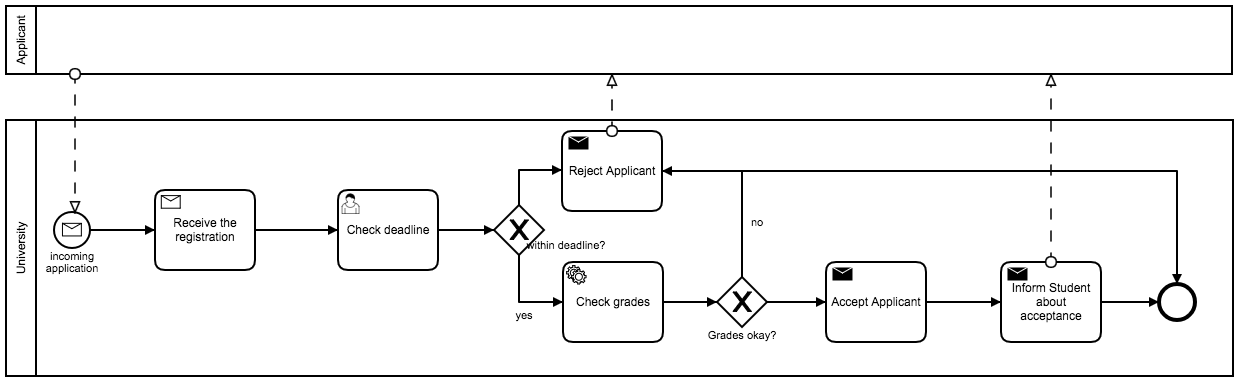
\includegraphics[scale=0.5]{../figures/chapter_indicators/BPMN_Example_Student_Application.png} 
		\caption{A small BPMN example: the application process for study programs.}
	\label{fig:BPMNex}
\end{sidewaysfigure}

Business Process Model and Notation incorporates the term \textit{Business Process}, which has been defined and redefined many times by today. For this thesis, we use the OMG's definition of business processes: 

\begin{quote}
Business Processes: business plans include Courses of Action - what the enterprise has to do to achieve its Ends - transformed into Business Processes that ecnompass activities, sequencing, dependencies, interactions, triggering by business events, etc. \cite{bmm2015}
\end{quote}

Business processes are ways to achieve goals, to align activities along them and to define interactions, decisions and events. This definition basically incorporates all the core elements of BPMN: Activities, paths, swimlanes (for responsibilities), decisions and events. To recap the notation of BPMN, a small example is shown in figure \ref{fig:BPMNex}. 
In this model, the application process for a student program is shown, which consists of tasks, for instance \textit{Receive the registration} or \textit{Check deadline}. Tasks can be precised as \textit{Manual tasks}, \textit{Send / Receive Tasks} and have assignees, as shown in \textit{Check deadline}. In current Workflowmanagementsystems, this workflow model can be fully automated and the assignee is presented its tasks when they are instantiated, in example when an application form was received. BPMN models have a starting and an end point which can also be events. In our example, the starting point is a \textit{Message Event}, that indicates the process has started due to a received message. \\
Another major concern in every control flow oriented modeling language are decisions. BPMN models usually consist of several decision points, depict as diamond-shaped \textit{Gateways}, either empty or with a special symbol inside. Each symbol stands either for \textit{AND}, \textit{OR}, \textit{XOR} or \textit{COMPLEX}. They direct the control flow depending on the decision logic prescribed. In our example, a \textit{XOR} Gateway guide the control flow into either the direction of acceptance or the opposite one, depending on what date the applicant's form was submitted. Additionally, the communication between the workflow's two participants is notated as so called \textit{Pools}, which can be divided into \textit{Swimlanes}. Each pool is a communication partner and a swimlane indicates different responsibilities, such as departments. If a pool is not filled with BPMN elements, the communication partner is out of scope of the modeler and the processes cannot be modeled. These pools are \textit{Black boxes}. 

As we see in the example, the process is structured and completely predefined, thus has no room for creative decisions or even planning at run-time. The only way the process can differ is human intervention or changing the process at design-time. The former is equal to not executing the process in the intended way and the latter is bad for processes in volatile environments. BPMN is suited for a limited variety of processes, foremost business processes and processes and derivatives. The OMG's specification excludes specifically the following \cite{BPMNspec}: 

\begin{quote}

\begin{itemize}
\item Definition of organizational models and resources,
\item Modeling of functional breakdowns,
\item Data and information models,
\item Modeling of strategy,
\item Business rules models
\end{itemize}

\end{quote}

%Although excluded, data and information can be modeled by artifacts. It's not like an \textit{Unified Modeling Language} (UML) model where classes and inheritance is mapped, but it is useful to handle forms and different kind of documents which need to be passed along the tasks. 
%For business rules, this is also applicable. BPMN contains a special form of tasks called \textit{Business Rule Task}, which "[...] provides a mechanism for the Process to provide input to a Business Rules Engine and to get the output of calculations that the Business Rules Engine might provide" \cite{BPMNspec}. Business Rule Tasks are predestined for small spreadsheets fed injected into a business rule engine, which is usually a Java class. It is easy to use and implement, since the Business Analyst files a spreadsheet and the developer uses the CSV-file to implement the business rule engine. This procedure, however, works only at design-time and not at run-time, which is a downside being discussed in a subsequent section about DMN. 

Furthermore, the OMG's specification not only provides exclusions such as the ones mentioned above, but it helps to indicate the correct usage of BPMN. Derived from the background chapter \ref{chapter:background} and the example above, the following indicators (table \ref{tab:bpmnIndicatorsTable}) serve as a guidance for modelers to identify when to use BPMN correctly. 

% Please add the following required packages to your document preamble:
% \usepackage{booktabs}
\begin{table}[]
\centering
\begin{tabular}{@{}ll@{}}
\toprule
Indicators                   & BPMN                                    \\ \midrule
Documentation style          & Directives                              \\
Preceding process map        & Flowchart                               \\
Characteristics of work      & Routine, predictable, automatable       \\
Characteristics of process   & Rigid, predefined, workflow-centric     \\
Characteristics of decisions & Simple (either / or)                    \\
Control flow                 & Definite control flow, required         \\
Intervention at run-time     & No                                      \\
Objective                    & Automated workflow execution            \\
Type of process              & Business process                        \\
Typical application          & Billing, Accounting, Assembly-line work \\ \bottomrule
\end{tabular}
\caption{BPMN indicators.}
\label{tab:bpmnIndicatorsTable}
\end{table}

%Information about processes is often stored in documents, deprecated models or held by knowledge carriers according to Dumas et al. \cite{Dumas2013}. This information needs to be extracted by the application of the so called \textit{Process Discovery}, which is in short gathering all the information in a technical or manual way before creating the models. Having this information gathered together, the key question before modeling is \textit{Does the work consist of routine elements which can be optimized or even automated?} (see \ref{tab:bpmnIndicatorsTable}). 
Routine processes occur regularly and their flow is "known a priori" according to \cite{Zeising_2014}. Consequently it is not intended to change the process flow during run-time, as routine are well-structured and predefined.\\
In our example, the decisions are simple yes or no questions. One of them, \textit{Check grades}, is a business rule task containing a small table of when a grade is acceptable or must be rejected. Overall, the decisions do not require modeling any requirements or personnel apart from the assignee involved in the decision making process. Furthermore, the decisions are always stuck with rules or events that happened before. The process itself is control-flow-oriented and the control flow is required and definite since every candidate needs to be processed in a fair and equal manner. In the end, the process could be automated completely with the appropriate workflow management system and would not need any assignee to check the deadline or the grades. \\
Overall, BPMN processes are intended to be predictable and to capture routine work. As a matter of fact, a process model's object is either optimizing or automating a process. In terms of BPMN, the automation of routine work is the main objective although it is not always possible to fully automate business processes. \\
The given example lacks the documentation and the preceding process map. Both are key artifacts to determine the modeling language, because each contains meta information about the process. Since BPMN processes are often predefined and orchestrated, meaning someone in the company fully designs the process without intended deviation, the documentation resembles directives that are also fully specified and provide a guideline how to correctly execute a task. Directives provide a precise description and strict sequence of tasks along with exception handling and interfaces to different processes. BPMN's core elements are tasks, control flow, events and gateways that are intended to capture the directives and make them executable for machines and human interaction. \\
A typical application is a billing process or assembly-line work that, in a big picture, result in a certain output creating a value for the company. A billing process can involve several departments and persons of responsibilities. However, every iteration of the process is intended to provide a similar, predictable output and a fully repeatable execution. \\
It is to say that BPMN and DMN resemble a lot when it comes to indicators. The goal of DMN was to create a modeling technique that incorporates both, decision logic and the declarative illustration of dependencies as well as authorities for a decision (see DMN section). The goal was also to create a data handling modeling technique with the ability to process complex rules and data points. Apparently, these decisions are also routine ones and predictable up to a certain point. The main difference between DMN and BPMN is that DMN is not able to capture workflows and BPMN is not able to capture data processing. As a matter of fact, a combined approach of both modeling techniques might in almost every case suitable due to the complementary aspect of DMN \cite{DMNspec2016}. 

\section{CMMN and knowledge work}
Routine work occurs in every company, every industry and even in our leisure time. However, not every job is comprised entirely of routine work.
\\
If a person is sick and needs to see the doctor, often the doctor's job consists of routine parts and ad hoc parts. Each patient suffers in a different way, has a private or statutory health insurance, is able to understand the doctor's language or not. In each case, the doctor or the medical personnel needs to decide depending on the situation to identify the patient's disease and medicate him accordingly. Overall, this job requires more knowledge and experience than a strict workflow. Applying the BPMN indicators makes the necessity of a different modeling technique obvious as the indicators do not meet the requirements of this example (adaptable instead of a definite workflow, knowledge-centric process instead of worklflow-centric).\\
Standardized by the OMG in 2014 \cite{CMMNspec2014}, the modeling language is intended to meet the requirements of knowledge intensive professions and support workers with models and their execution in workflow management systems. 
The above described example diverges from the business processes explained in the BPMN section earlier. Instead of focusing on what \textit{has} to be done in which order, the medical personnel should adhere to what \textit{can} be done, as Van der Aalst et al. described in \cite{aalst2005}. This is an essential part of the \textit{Case Management} (CM) and \textit{Adaptive Case Management} (ACM) approach. Case management starts with a case such as a legal case, a patient's disease or "some other focal point around which actions are taken to achieve an objective" \cite{CMMNspec2014}. As a matter of fact, a case can also be a project that has to be managed or an event that needs to be organized. \\
Each case contains a set of tasks and files necessary to achieve the goal. These sets are "minimally predefined" \cite{CMMNspec2014} resulting in two phases of working with cases: the design phase and the running phase \cite{CMMNspec2014}. During the design phase, tasks and information are aggregated in a manner that is very similar to business process designs. As a result, the work is available in a more structured way as it has been before, yet with the possibility to perform the work completely situation-dependent, if necessary. Case management requires the run-time flexibility such as performing tasks depending on the situation, changing the order of tasks or even collaborate with different people involved as intended. 
At a first glance, this seems counter-intuitive to the common understanding of modeling processes, which is presumably modeling business processes or similar strictly structured ones. To illustrate the paradigm of case management and introduce the CMMN notation, figure \ref{fig:CMMNex} provides an example. The subsequent explanation is derived from \cite{CMMNspec2014} and \cite{hinkelmann2015}.

\begin{sidewaysfigure}

	\label{fig:CMMNex}
	\centering
	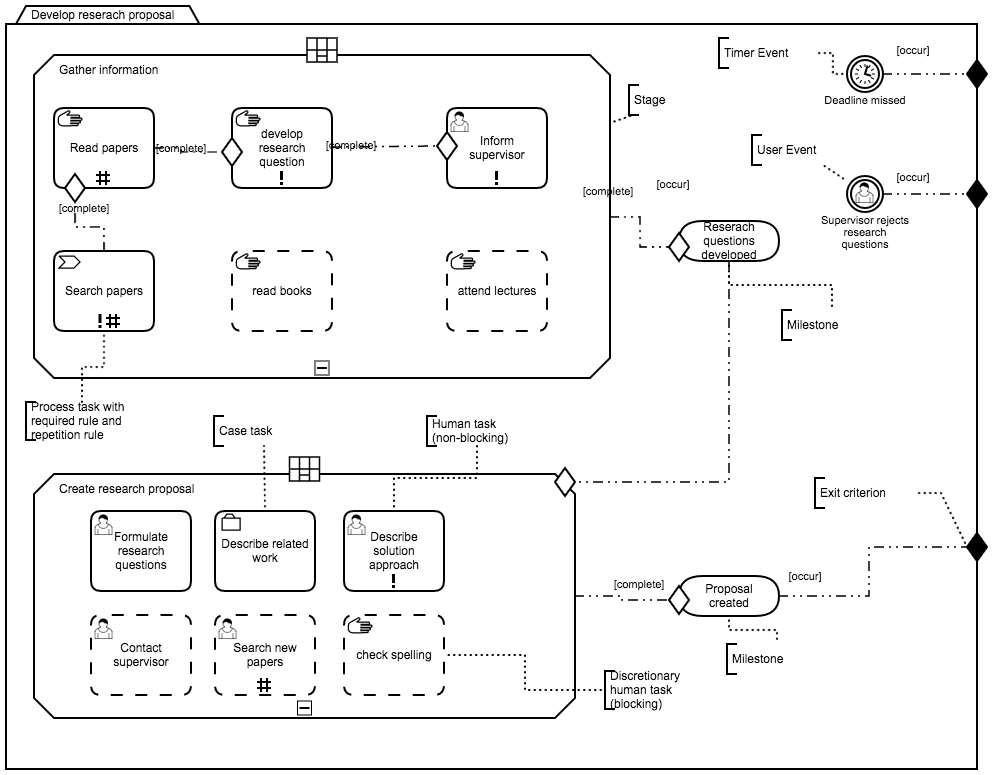
\includegraphics[scale=0.5]{../figures/chapter_indicators/CMMN_Example_Proposal_Creation.png} 
		\caption{CMMN example: Creating a research proposal.}
\end{sidewaysfigure}

The first element that immediately catches the eye in this example is a large folder depicting the \texttt{Case Plan Model}, a root element containing all further elements involved with a name tag in the upper right corner. Next, there is a big structure called a stage and illustrated as a rectangle. Similar to BPMN, stages form a group of elements into a sub process or - to put it in the CMMN context - in a sub case. Stages can be connected via sentries and connectors that are the lines between tasks and the diamond shaped exit or entry criteria. Both, exit and entry criteria trigger when events occur. There are three rules to make sentries trigger:

\begin{itemize}
\item \texttt{on [event] if [condition]} 
\item \texttt{on [ event]}
\item\texttt{if  [condition]}
\end{itemize}

According to the CMMN specification, this provides the opportunity to receive events and check whether they have effect on the following process steps \cite{CMMNspec2014}. \\
In figure \ref{fig:CMMNex}, a timing event is called \textit{Deadline missed}. This event is connected to an exit criterion, denoted as a black diamond on the border of the Case Plan Model. When the event is triggered, the sentry checks \texttt{on [deadline missed] if [date today > deadline date]} and triggers the exit criterion terminating the case due to the missed deadline. A different event type is the \textit{User Event} listening to user interactions that trigger the exit criterion. Besides these two event types, each task, stage and \textit{Case File Item} can trigger events on their own which are received by sentries. \textit{Case File Items} are containers for pieces of information, for instance the patient's record or in this example the papers, which need to be read (not contained in the diagram). They are denoted as .\\
Another structural element is the \textit{Milestone}, an oval shaped form representing an "achievable target" \cite{CMMNspec2014} and providing the ability to measure the progress of a case. Each milestone can have multiple entry criteria or none to show that a milestone is reached or not. In general, "no work is directly associated with a milestone" \cite{CMMNspec2014} but rather a "completion of a set of tasks" or "the availability of key deliverables" \cite{CMMNspec2014}. \\
Figure \ref{fig:CMMNex} contains two example milestones: \textit{Research questions developed} and \textit{Proposal created}. Both milestones are connected to either a stage or an exit criterion indicating a dependency. The first milestone needs to be achieved to create the research proposal, the latter one determines the successful termination of the case. \\
As mentioned earlier, CM requires run-time flexibility and by now, there has nothing been explained but tasks, events and milestones which are per se inflexible. To guarantee run-time planning, tasks and stages have a discretionary version. Discretionary means, a user may decide during run-time if this task or stage will be executed in a following iteration. This mechanism makes it possible to model knowledge and experience combined with routine steps. In our example, the gathered papers might not be enough to provide good citations and emphasize the solution approach. Here, only the case worker can identify if he needs to do more research to find correct citations, as this is a decision requiring knowledge and experience in writing research papers. It is to his or her discretion if the task will be executed or not. \\
Supplementary to \textit{Discretionary Items}, \textit{Planning Tables} indicate the ability to plan Discretionary Items and apply control mechanisms called \textit{Applicability Rules}. Case workers are presented \textit{Planning Items} if the corresponding Applicability Rule evaluates to true. Overall, this allows the modeler and the case workers to plan at design-time (creating the case model) and at run-time (planning the time discretionary items). 
The last visible part of the CMMN notation, that has not been explained, is the type of tasks available. In the example case, there are four types of tasks (each type can be indicated in the upper right corner of the task):

\begin{itemize}
\item \textit{Human Tasks} either blocking (indicated with a "User" in the upper right corner) or non-blocking with a hand in the right corner
\item \textit{Process Task} with a "Chevron" symbol 
\item \textit{Case Task} with a folder symbol 
\end{itemize}

Both Human Tasks indicate that an assignee with the appropriate role needs to fulfill the modeled work here. \textit{Non-blocking} signifies this step can be done while other tasks of the model run simultaneously in contrast to the blocking one, which does not allow other tasks to be performed at the same time. A \textit{Process Task} calls a business process modeled, for example, in BPMN and a \textit{Case Task} calls a different case handing over input parameters and demanding an output. \\
In figure \ref{fig:CMMNex}, \textit{Read Papers} is a non-blocking human task, \textit{read books} a non-blocking discretionary human task, \textit{Formulate research questions} a blocking human task, \textit{Describe related work} a case task and \textit{Search papers} a business process task.
Apart from the mentioned types of tasks, there a additional execution semantics as seen in the \textit{Search papers} task. An exclamation mark signifies this task as to perform, a sharp that this task has several iterations and a play symbol indicates the \textit{Manual Activation Rule} (not in the example). This rule is connected to entry criteria and transitions from the status \texttt{enabled} to \textit{active} if the criterion's condition is fulfilled. 
CMMN, in contrast to BPMN, offers a complete lifecycle with corresponding states.

\begin{figure}
  \centering
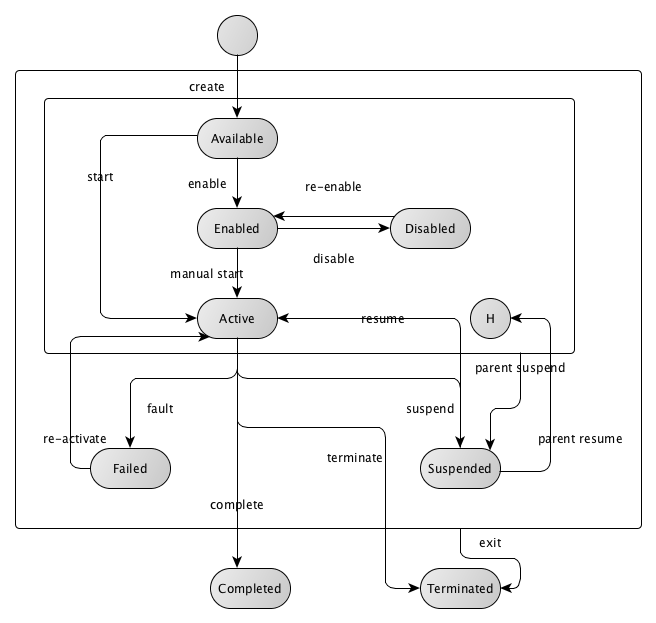
\includegraphics[width=0.7\textwidth]{../figures/chapter_indicators/CMMN_Stage_and_Task_Lifecycle_CMMN.png} 
\caption{Stage and Task Lifecycle adopted from Figure 7.3 in the CMMN specification \cite{CMMNspec2014}.}
  \label{fig:CMMNstates}
\end{figure}

Figure \ref{fig:CMMNstates} is a replica of Figure 7.3 in \cite{CMMNspec2014} and shows the different states and transitions for stages and tasks. These stages, compared to BPMN, allow the modeler and the worker to measure and plan work in a different way than business processes are handled. One of the most commonly mentioned downsides of BPMN is the lack of states and transitions according to \cite{Recker2010}. In the example (Fig. \ref{fig:CMMNex}), states are not included since they are not visible in the notation and only occur during run-time. In addition to Fig. \ref{fig:CMMNstates}, CMMN offers similar states for sentries and the whole case plan model and can be found in the execution semantics chapter in \cite{CMMNspec2014}. \\

% Please add the following required packages to your document preamble:
% \usepackage{booktabs}
% \usepackage{graphicx}
% \usepackage[normalem]{ulem}
% \useunder{\uline}{\ul}{}
\begin{table}[]
\centering
\resizebox{\textwidth}{!}{%
\begin{tabular}{@{}ll@{}}
\toprule
Indicators                   & CMMN                                                 \\ \midrule
Documentation style          & Descriptions of best practices and recommendations   \\
Preceding process map        & Cluster                                              \\
Characteristics of work      & Agile, emerging, not automatable                     \\
Characteristics of process   & Adaptive, partly predefined, knowledge-centric       \\
Characteristics of decisions & Stateful (transition form one to another state)      \\
Control flow                 & Indefinite control flow, optional                    \\
Intervention at run-time     & Yes                                                  \\
Objective                    & Support manual work                                  \\
Type of process              & Case                                                 \\
Typical application          & Reviews, Medical attendance, Managing and organising \\ \bottomrule
\end{tabular}%
}
\caption{CMMN indicators.}
\label{tab:CMMN_indicators}
\end{table}

Table \ref{tab:CMMN_indicators} summarizes the notation's characteristics and classifies them as indicators. In the earlier examples we saw that CMMN is suitable for agile and partly predefined work. The worker's knowledge is crucial during execution phase, whereas workflows and sequences are less important. Compared to BPMN, CMMN captures the flexibility of processes that require situation-dependent decisions, agile work whose tasks emerge during run-time and cannot, or at least to a small extent, predicted and thus predefined during design-time. Furthermore, decisions are stateful due to rules and sentries and function as monitoring tools instead of sequencing work. This leads to a flexible control flow, only describing the dependencies of task or milestones that need to be achieved in order to fulfill the whole case. \\
CMMN documentation and process maps might resemble best practices or descriptions of work, as the content of cases often diverges. However, process discovery should lead to some extent of a description, what can be done to achieve the case and what are the key elements that need to be modeled. Following this, process mapping would rather result in an aggregation of tasks that belong together instead of a flowchart indicating steps and sequences. \\
Overall, BPMN and CMMN differentiate in many points and capture completely different settings. Whereas BPMN has the objective to automate processes, CMMN is intended to support workers by automating certain steps or simplifying the monitoring of case. This makes it a declarative modeling technique according to \cite{FahlandLuebkeMendlingEtAl2009}. 

%Table \ref{tab:cmmnIndicatorsTable} shows a summary derived from the explanation and the example, both planting on the basis of the CMMN specification \cite{CMMNspec2014}. The example emphasized that CMMN is in general applicable for not predefined, to a high degree knowledge dependent work. Decisions are modeled in conditions on when to enter or exit stages, task or milestones. Rules such as \textit{Application Rule} or \textit{Repetition Rule} allow the modeler to guide the case worker through tasks and show him or her what tasks have to be done and which have to be done for a specific amount of iterations. However, decisions similar to gateways in BPMN are not in scope of this notation and dedicated to the case worker. In addition, the required flexibility is fulfilled by \textit{Discretionary Items} allowing the workers with the appropriate role to adapt the workflow in during run-time. States as shown in figure \ref{fig:CMMNstates} contribute to this flexibility but also let the involved personnel measure the progress of each case. This results in a more manageable and verifiable way of Case Management. 

\section{DMN and decision making}
In section \ref{section:BPMNindicators}, decision-making in BPMN was shown with the aid of a small example, whose excerpt is shown in figure \ref{fig:BPMNshortenedApplicationEx}. Two gateways guide the control flow according to the decisions made. Each gateway compares a value with a given limit and verifies it. If the value is correct, the control flow passes on to the next gateway or, in case the value is out of bounds, rejects the student's application. TThese are simple \textit{either or} questions. \\
Figure \ref{fig:BPMNexpandedApplicationEx} demonstrates a more sophisticated version of the same process. To pass the application process,  one of the four requirements needs to be fulfilled. Each requirement is implemented as a gateway that checks if the applicant either fulfills it or not. All of the gateways are \texttt{OR} gateways signalizing a lose decision making compared to \texttt{XOR} gateways. At a first glance, figure \ref{fig:BPMNexpandedApplicationEx} looks more complicated than figure \ref{fig:BPMNshortenedApplicationEx}. Although the actual decision-making process is kept simple, the BPMN notation with its gateways makes it look confusing and, at a much larger scale, for the reader impossible to comprehend the process as a whole. At this point, DMN becomes relevant. 

\begin{sidewaysfigure}
  \centering
    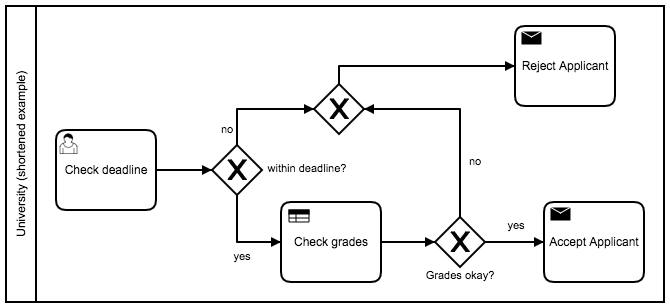
\includegraphics[scale=0.5]{../figures/chapter_indicators/BPMN_Example_Student_Application_Short.png}
    \caption{Shortened example from section \ref{section:BPMNindicators} with only two decisions.}
  \label{fig:BPMNshortenedApplicationEx}
    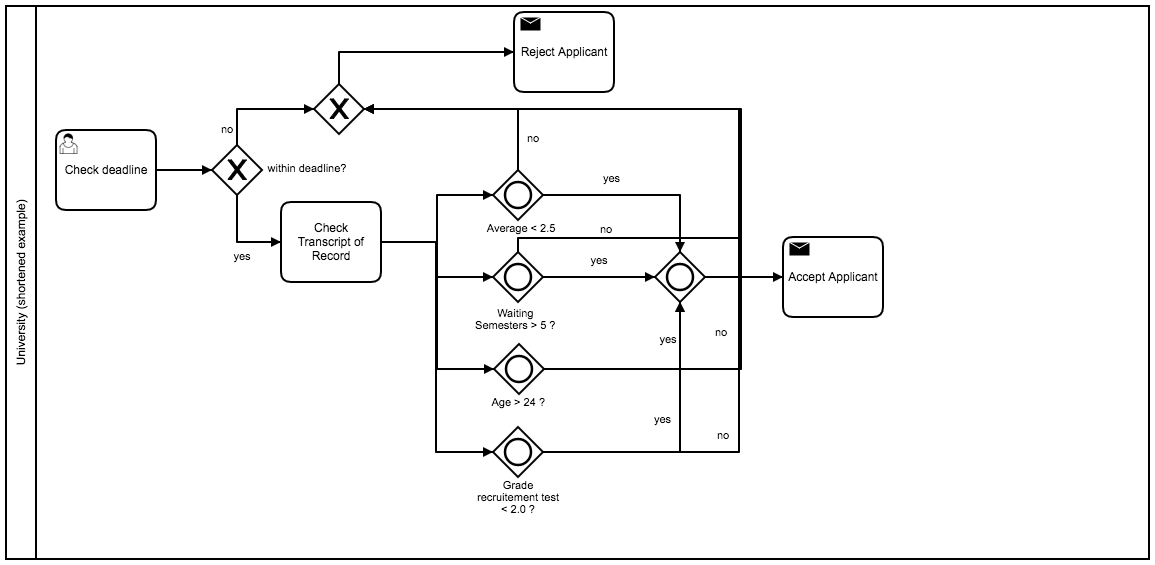
\includegraphics[scale=0.4]{../figures/chapter_indicators/BPMN_Example_Student_Application_DMN_Short.png}
    \caption{Shortened example from section \ref{section:BPMNindicators} with additional decisions.}
  \label{fig:BPMNexpandedApplicationEx}
\end{sidewaysfigure}

\begin{figure}
\begin{center}
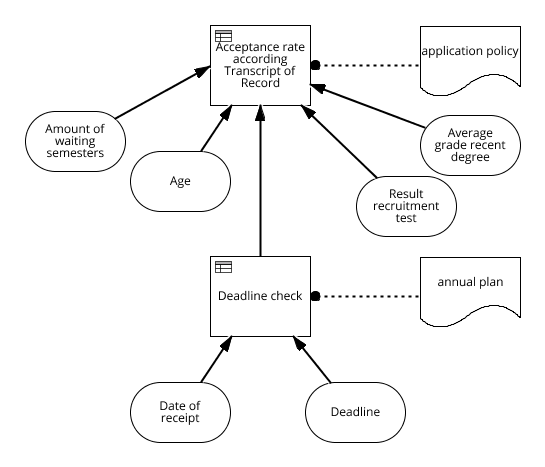
\includegraphics[width=0.5\textwidth]{../figures/chapter_indicators/DMN_Application_Example_Deadline_ToR.png} 
\end{center}
\caption{A DMN Decision Requirement Graph incorporating the decision-making of the BPMN process in \ref{fig:BPMNexpandedApplicationEx}.}
\label{fig:DMN_DRD_Application}
\end{figure}

The DMN notation comprises two parts: the \acl{DRG} with one ore more \aclp{DRD} and the decision tables. Figure \ref{fig:DMN_DRD_Application} illustrates the corresponding \ac{DRG} for the decision-making seen in Fig. \ref{fig:BPMNexpandedApplicationEx}.
\\
DMN's notation for DRDs contains only four distinct shapes and three different types of connectors, which can be seen in Fig. \ref{fig:DMN_DRD_Application}: 

\begin{itemize}
\item \textit{Decision}: Decisions are depicted as rectangles and incorporate the decision logic which is mapped in decision tables. In the example there are two decisions, \textit{Deadline check} and \textit{Acceptance rate according to Transcript of Record} and both have a table symbol in the upper right corner indicating the decision logic. 
\item \textit{Input Data}: Each decision needs inputs and \textit{input data} is the fundamental and least complex form possible. This element stores information of any type from simple types like dates and integers to lists and functions expressed via \acf{FEEL}. An \textit{Input Data} element may only be connected directly to decisions and knowledge sources. 
\item \textit{Knowledge Source}: DMN makes it explicit where knowledge sources are involved in the decision-making. Typically knowledge sources are documents, best practices but also people or bodies of legislation \cite{DMNspec2016}.  "Knowledge sources are the authorities for a decision [...]" \cite{DMNmicroguide}, which may be connected with input data since managers, for instance, might need background information not directly involved in the decision logic. In the example, the application policy and annual plan of the university is used as \textit{knowledge source}.
\item \textit{Business Knowledge Model}: In contrast to Knowledge Sources, Business Knowledge Models are non-authoritative and serve as container for analytic models, decision logic or business rules \cite{DMNspec2016}. It is depicted as a rectangle with cut-off corners in the upper left and lower right. As they only influence decisions directly, the specification allows consequently no connection but with decisions or different business knowledge models. Due to the shortness of the example, Business Knowledge models are not contained in Figure  \ref{fig:DMN_DRD_Application}. 
\end{itemize}

As stated above, the notation comprises only four elements making it a very compact modeling language in terms of the \ac{DRG}. In addition, there are three different connectors indicating either an \textit{information requirement} (connections from decisions to decisions or input data to decisions), an \textit{authority requirement} (connections from knowledge models to decisions, business knowledge models or different knowledge sources) or \textit{knowledge requirement} (connections from business knowledge models to decisions or different business knowledge models). 

\begin{sidewaysfigure}
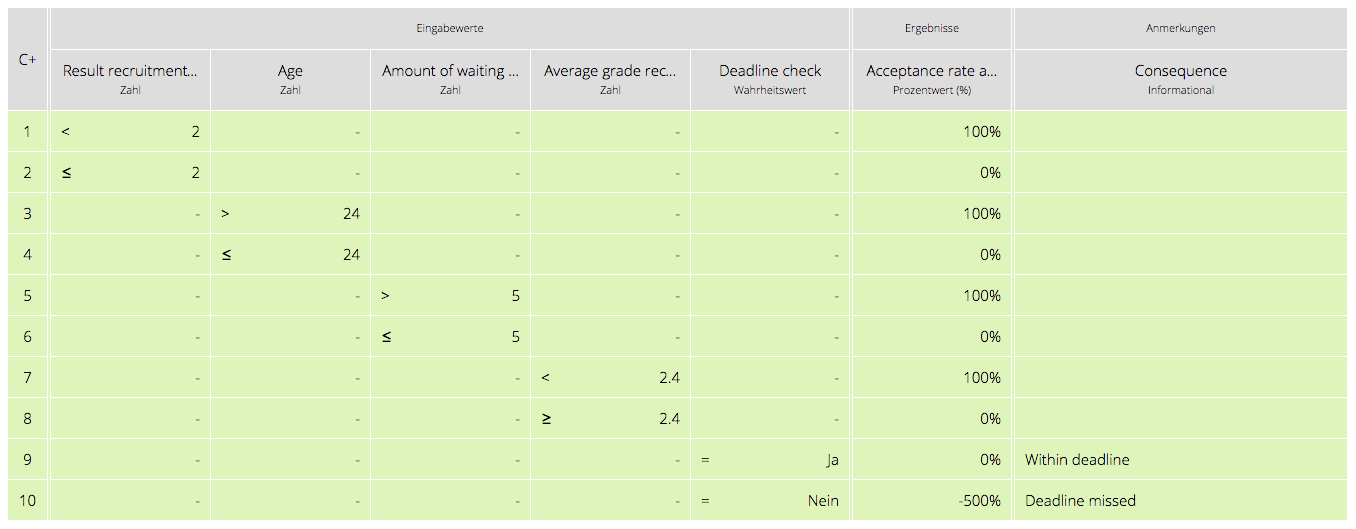
\includegraphics[width=\textwidth]{../figures/chapter_indicators/DMN_Application_Example_Decision_Table_ToR.png} 
\caption{An example DMN decision table with the decision logic accord to the BPMN example in Fig. \ref{fig:BPMNexpandedApplicationEx}.}
\label{fig:DMN_decision_table_application}
\end{sidewaysfigure}

The second part of the DMN specification allows the modeler to create decision tables containing the decision logic. An example table \footnote{Each modeling tool implementing the DMN specification is allowed to vary the orientation of decision tables and the concrete look, such as colors or shades.} is provided in Figure \ref{fig:DMN_DRD_Application} implementing the decision logic according to the BPMN example in Figure \ref{fig:BPMNexpandedApplicationEx}. Each table is comprised of several input columns and at least one output column. An input can be a string, integers, floats or basically any type of numbers or enumerations. In this example table, there are five input columns and one output column with annotations such as \texttt{Deadline missed}. Each row signifies a rule in the following syntax: \texttt{If [INPUT A] AND [INPUT B] then [OUTPUT C]} \cite{DMNspec2016}. The inputs are logically connected by the boolean \texttt{AND}-operator resulting in as many outputs as desired, if a rule matches. For every input in the decision table, there is an \texttt{input data} element modeled in the related \ac{DRG}. This also applies for decisions and sub-decisions. \\
Comparing the table with the BPMN example demonstrates a downside of the decision table: the "\texttt{AND} only" syntax. However, modeling \texttt{OR} connections is possible with a workaround. Besides the table's data and rules, business analysts can also define \textit{hit policies}. These policies are necessary if some of the rules overlap. In the example table (Fig. \ref{fig:DMN_DRD_Application}), all of the rules are intended to overlap making a hit policy necessary. There are two major categories of policies: \texttt{single hit} and \texttt{multiple hit}. The former one allows only to trigger one rule, the latter one allows several rules to trigger. A brief overview with an explanation can be found in table \ref{tab:DMN_hit_policies}. 

% Please add the following required packages to your document preamble:
% \usepackage{booktabs}
% \usepackage{graphicx}
\begin{table}[]
\centering
\resizebox{\textwidth}{!}{%
\begin{tabular}{@{}ll@{}}
\toprule
Policy       & Variations                                                                                                             \\ \midrule
Single hit   & Unique (no overlap allowed)                                                                                            \\
             & Any (overlap allowed, outputs must be equal)                                                                           \\
             & Priority (returns matching rule with highest output priority)                                                          \\
             & First (first hit by rule order)                                                                                        \\
Multiple hit & Output order (returns all hits in decreasing output priority order)                                                    \\
             & Rule order (returns all hits in rule order)                                                                            \\
             & \begin{tabular}[c]{@{}l@{}}Collect (aggregates all hits with specified operators:\\ sum, min, max, count)\end{tabular} \\ \bottomrule
\end{tabular}%
}
\caption{DMN hit policies cited from the DMN specification \cite{DMNspec2016}.}
\label{tab:DMN_hit_policies}
\end{table}
 
To achieve an \texttt{OR} connection of the rules, the hit policy \todo{DMN Tabelle probieren auf Englisch umzustellen} is set to \texttt{Multiple Hit: collect (sum)} and the measuring unit of the output is set to percentage. Consequently, the acceptance rate is measured in percentage. The applicant is able to achieve zero or more than 100 percent according to the \texttt{collect: sum} rule. Another problem of this method is the inflexibility of the outputs. In this example, an output value of \texttt{true} or \texttt{false} would have been the best way to model the decision, but neither the decision table nor \ac{FEEL} allow the aggregation of boolean values. \\
To individualize the decision logic or create more advanced rules, the DMN specification aggregated several functions and types into an expression language called \acl{FEEL}. It is similar to \ac{SQL} and \ac{PMML} making it easier to understand for non-developers. The expression used in the \texttt{deadline check} table is also a predefined function with two inputs (deadline date and date of receipt) and a range of numbers implemented implemented as two rules: \texttt{DayDiff(Date of receipt, Deadline)}. \\
Last of all to mention is the sub-decision \texttt{Deadline check}. The decision logic is not implemented in this table, but is referenced by a another decision table (see Fig. \ref{fig:DMN_DRD_Application} for illustration). A simple check written in \ac{FEEL} counts the difference between the application's date of receipt and the given deadline. If the result is less then zero, the deadline is missed and the output of \texttt{Deadline check} is \texttt{false}. Otherwise, if the result equals zero or more, it evaluates to \texttt{true}. \\

In review, the examples illustrated the multiple uses of the DMN language. Decision tables are useful for automating data intensive decisions and replacing vast BPMN gateway trees. In the same way it is possible to model decisions that require rather knowledge, best practices or analyses than a large amount of data by skipping the decision logic part and only define the dependency graph. 
On the contrary, it is not possible to any sequence with the DMN notation but the dependency of decisions or the amount of iterations. Although the specification emphasizes the independence of the the notation \cite{DMNspec2016}, the \ac{DRG} on its own might have few useful cases pf application where a standalone \ac{DRG} is the most convenient solution. \\

% Please add the following required packages to your document preamble:
% \usepackage{booktabs}
% \usepackage{graphicx}
\begin{table}[]
\centering
\resizebox{\textwidth}{!}{%
\begin{tabular}{@{}ll@{}}
\toprule
Indicators                   & DMN                                                       \\ \midrule
Documentation style          & Spreadsheets                                              \\
Preceding process map        & Decision trees                                            \\
Characteristics of work      & Decision-intensive, predictable, automatable              \\
Characteristics of process   & Predefined, adaptive, data-centric                        \\
Characteristics of decisions & Complex (data processing)                                 \\
Control flow                 & Dependencies, required                                    \\
Intervention at run-time     & Yes                                                       \\
Objective                    & Automated data processing                                 \\
Type of process              & Decisions                                                 \\
Typical application          & Calculation of discount rates, salary, choosing assignees \\ \bottomrule
\end{tabular}%
}
\caption{Indicators for the identification of DMN use cases.}
\label{tab:DMN_indicators}
\end{table}

Table \ref{tab:DMN_indicators} summarizes the knowledge acquired by analyzing the DMN specification \cite{DMNspec2016}, Debevoise and Taylor \cite{DMNmicroguide} and \cite{BiardMauffBigandEtAl2015a}, as well as creating the provided examples in this section. It was shown that DMN is an applicable solution for processes that focus on decisions or require decisions, thus are complex to illustrate in BPMN. The most common applications are calculations of salaries, provided in \cite{DMNspec2016} or making a choice by several influencing factors, for instance choosing the right vehicle for hazardous material \cite{DMNmicroguide}. Particularly the breakdown into two parts, the \acl{DRG} and the decision tables, makes it simple for the modeler to decide between decisions that only need data, therefore use the decision table, model the dependencies of decisions and the decision-makers, ergo utilize the \ac{DRG}, or combine both. \\
Table \ref{tab:DMN_indicators} also shows a similarity to BPMN: Both modeling approaches aim at the automation of their domains. BPMN's objective is to automate workflows, whereas DMN provides the ability to automate decisions. Both notations capture routine work that is mostly predefined. In addition to that, DMN provides the ability to adapt values of the decision logic during run-time. How this is exactly achieved depends on the implementation by the corresponding software tool. Camunda, for example, provides a \ac{REST} API that allows the users to create or delete decisions during run-time. \\
The main difference between DMN and BPMN, however, is what they are able to capture. DMN is a notation that only is able to process data and outputs a decision that can be handled by other modeling languages, if desired. BPMN is also able to handle decisions, but not to process data in the way DMN does. This is emphasized by the control flow of the DMN language: decisions can enhanced with dependencies and knowledge sources. Overall, DMN is a notation that only serves for decisions and does not suit for any different use case. \\
Data that needs to be processed to find a decision is often stored in spreadsheets instead of free text documents. This is a strong indicator for DMN, since the spreadsheets can be copied in DMN's decision logic. Furthermore, decisions that have sub-decisions or dependencies might be clustered in a decision tree during process discovery. The \ac{DRD} is able to  incorporate these decision trees and make them executable. \\
In Chapter \ref{chapter:combination}, the combination of DMN and BPMN is described along with use cases where DMN suits as a replacement for gateways and a functions as a data processor or event-handler. This chapter describes the complementary character of the DMN notation as well.

\section{Summary}
In this chapter, each specification was presented with examples and their characteristics. By analyzing the OMG's standards and further research publications, these characteristics could be transformed into indicators helping modelers to identify when to use the corresponding technique. Additionally, the examples explained the fundamental principles of the notations and how to use them correctly. The main focus, however, was developing the indicators. For further information about the notations and more sophisticated examples or instructions, please refer to the corresponding OMG specification or the provided sources in the references chapter. 
Additionally, a recommendation of how to combine manual process discovery techniques was presented along with an explanation of each approach. Besides the manual discovery, the automated one was explained and a recommendation for a corresponding tool was stated. 
Concluding the indicator sections, BPMN is useful for predefined processes, mainly mapping routine work without the possibility for run-time intervention; CMMN is suitable for people working in volatile environments with routine parts but mainly work depending on their personal experience and knowledge; and DMN is a valuable way to encapsulate complex, data-intensive decision-making in a separate, compact notation that allows run-time adjusting. For all of the mentioned notations, there are overlaps that make it possible to combine them and creating a whole model with separate notations for each domains. This will be discussed more detailed in the following chapter.

\listoftodos
